% generated by scripts/pkl_to_latex.py
% source PKL : uscan_v1_L8_Ne8_t1_mode-uniform_nmin2_solver-gcg_full_restarts8_iter200_kmax4_tol1em09_U1to20_N20-d03a74da789e.pkl
% scan type  : uscan
% state      : gs
% quantity   : linear-entropy
% requires   : \usepackage{pgfplots} \pgfplotsset{compat=1.18}
% colours match the matplotlib PDF (tab10 cycle)
\definecolor{gmeC0}{HTML}{1F77B4}
\definecolor{gmeC1}{HTML}{FF7F0E}
\definecolor{gmeC2}{HTML}{2CA02C}
\definecolor{gmeC3}{HTML}{D62728}
\definecolor{gmeC4}{HTML}{9467BD}
\definecolor{gmeC5}{HTML}{8C564B}
\definecolor{gmeC6}{HTML}{E377C2}
\definecolor{gmeC7}{HTML}{17BECF}

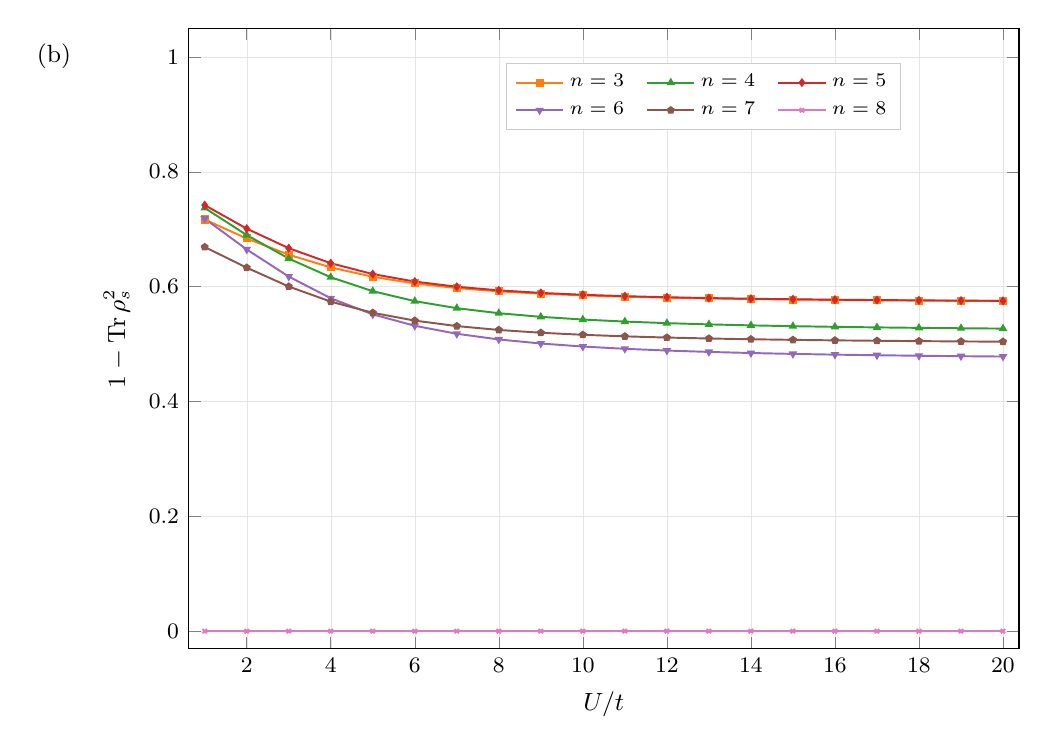
\begin{tikzpicture}
  \begin{axis}[
    width=\columnwidth,
    height=0.78\columnwidth,
    xlabel={$U/t$},
    ylabel={$1-\mathrm{Tr}\,\rho_s^2$},
    grid=both,
    grid style={line width=.1pt, draw=gray!20},
    tick label style={font=\footnotesize\rmfamily, /pgf/number format/fixed},
    label style={font=\small\rmfamily},
    scaled ticks=false,
    legend style={font=\scriptsize\rmfamily, draw=gray!40, at={(0.5,1.03)}, anchor=south, /tikz/every even column/.append style={column sep=6pt}},
    legend cell align={left},
    legend columns=3,
    ymin=-0.03,
    ymax=1.05,
    xmin=0.62,
    xmax=20.38,
    legend style={at={(0.620,0.890)}, anchor=center, fill=white},
    after end axis/.append code={\node[anchor=east, font=\small\rmfamily] at (axis description cs:-0.13,0.954) {(b)};},
  ]
    \addplot[color=gmeC1, mark=square*, mark size=1.1pt, line width=0.7pt] coordinates {
        (1,0.716899) (2,0.683835) (3,0.655627) (4,0.633456)
        (5,0.617121) (6,0.605564) (7,0.597491) (8,0.59181)
        (9,0.587738) (10,0.584753) (11,0.582515) (12,0.580799)
        (13,0.579459) (14,0.578393) (15,0.577532) (16,0.576828)
        (17,0.576244) (18,0.575755) (19,0.575341) (20,0.574987)
    };
    \addlegendentry{$n=3$}
    \addplot[color=gmeC2, mark=triangle*, mark size=1.1pt, line width=0.7pt] coordinates {
        (1,0.736984) (2,0.689842) (3,0.648909) (4,0.616323)
        (5,0.592064) (6,0.574715) (7,0.562453) (8,0.55372)
        (9,0.547387) (10,0.542696) (11,0.539144) (12,0.5364)
        (13,0.534241) (14,0.532514) (15,0.531112) (16,0.52996)
        (17,0.529001) (18,0.528195) (19,0.527511) (20,0.526926)
    };
    \addlegendentry{$n=4$}
    \addplot[color=gmeC3, mark=diamond*, mark size=1.1pt, line width=0.7pt] coordinates {
        (1,0.741871) (2,0.701) (3,0.666943) (4,0.640749)
        (5,0.621883) (6,0.608797) (7,0.599793) (8,0.593524)
        (9,0.589063) (10,0.585809) (11,0.583376) (12,0.581517)
        (13,0.580066) (14,0.578914) (15,0.577984) (16,0.577224)
        (17,0.576594) (18,0.576066) (19,0.57562) (20,0.575239)
    };
    \addlegendentry{$n=5$}
    \addplot[color=gmeC4, mark=triangle*, mark size=1.1pt, mark options={rotate=180}, line width=0.7pt] coordinates {
        (1,0.718368) (2,0.664724) (3,0.617543) (4,0.579732)
        (5,0.5517) (6,0.531818) (7,0.517882) (8,0.508025)
        (9,0.500918) (10,0.495677) (11,0.491724) (12,0.48868)
        (13,0.48629) (14,0.484383) (15,0.482838) (16,0.48157)
        (17,0.480516) (18,0.479631) (19,0.478882) (20,0.478241)
    };
    \addlegendentry{$n=6$}
    \addplot[color=gmeC5, mark=pentagon*, mark size=1.1pt, line width=0.7pt] coordinates {
        (1,0.668919) (2,0.633032) (3,0.600214) (4,0.57385)
        (5,0.554465) (6,0.540815) (7,0.531283) (8,0.524549)
        (9,0.519692) (10,0.516106) (11,0.513398) (12,0.51131)
        (13,0.509669) (14,0.508358) (15,0.507295) (16,0.506421)
        (17,0.505695) (18,0.505084) (19,0.504567) (20,0.504125)
    };
    \addlegendentry{$n=7$}
    \addplot[color=gmeC6, mark=x, mark size=1.1pt, line width=0.7pt] coordinates {
        (1,-0) (2,-0) (3,0) (4,0)
        (5,0) (6,0) (7,-0) (8,0)
        (9,0) (10,0) (11,0) (12,0)
        (13,0) (14,0) (15,-0) (16,0)
        (17,0) (18,0) (19,0) (20,0)
    };
    \addlegendentry{$n=8$}
  \end{axis}
\end{tikzpicture}
